\documentclass[12pt,a4paper]{article}
\usepackage[utf8]{inputenc}
\usepackage{amsmath}
\usepackage{listings}
\usepackage{verbatim}
\usepackage{graphicx} 
\oddsidemargin 0cm
\marginparwidth 0cm
\hoffset 0cm
\usepackage{polski}
\begin{document} 
\large
\begin{tabular}{|c|c|c|c|}
\hline
\multicolumn{4}{|l|}{Temat:}\\
\multicolumn{4}{|c|}{Rozwiązywanie układów równań liniowych metodami iteracyjnymi}\\
\hline
\multicolumn{1}{|l}{Wykonał:}&\multicolumn{1}{|l}{Wydział:}&\multicolumn{1}{|c}{Kierunek}&\multicolumn{1}{|l|}{Grupa:}\\
Marcin Fabrykowski&FiIS&Inf. Stos.&grupa 3\\
\hline
\end{tabular}
\normalsize
\vspace{2cm}
\begin{enumerate}
\item Metoda Jakobiego\\
Mając równanie Ax=b,\\
gdzie A=L+D+U,\\
przy czym:\\
\begin{equation}
A=\begin{bmatrix}
a_{11}&a_{12}&a_{13}\\
a_{21}&a_{22}&a_{23}\\
a_{31}&a_{32}&a_{33}
\end{bmatrix}=\
\begin{bmatrix}
0&0&0\\
l_{21}&0&0\\
l_{31}&l_{32}&0
\end{bmatrix}+
\begin{bmatrix}
d_{11}&0&0\\
0&d_{22}&0\\
0&0&d_{33}
\end{bmatrix}+
\begin{bmatrix}
0&u_{12}&u_{13}\\
0&0&u_{23}\\
0&0&0
\end{bmatrix}
\end{equation}\\
co po podstawieniu daje:\\
$Lx+Dx+Ux=b$\\
\begin{equation}
\begin{bmatrix}
0&0&0\\
l_{21}&0&0\\
l_{31}&l_{32}&0
\end{bmatrix}
\begin{bmatrix}
x_1\\x_2\\x_3
\end{bmatrix}+
\begin{bmatrix}
d_{11}&0&0\\
0&d_{22}&0\\
0&0&d_{33}
\end{bmatrix}
\begin{bmatrix}
x_1\\x_2\\x_3
\end{bmatrix}+
\begin{bmatrix}
0&u_{12}&u_{13}\\
0&0&u_{23}\\
0&0&0
\end{bmatrix}
\begin{bmatrix}
x_1\\x_2\\x_3
\end{bmatrix}=
\begin{bmatrix}
b_1\\b_2\\b_3
\end{bmatrix}
\end{equation}\\
przekszatałcając...\\
$Dx=b-(L+U)x$\\
\begin{equation}
\begin{bmatrix}
d_{11}&0&0\\
0&d_{22}&0\\
0&0&d_{33}
\end{bmatrix}
\begin{bmatrix}
x_1\\x_2\\x_3
\end{bmatrix}=
\begin{bmatrix}
b_1\\b_2\\b_3
\end{bmatrix}-
\left[
\begin{bmatrix}
0&0&0\\
l_{21}&0&0\\
l_{31}&l_{32}&0
\end{bmatrix}+
\begin{bmatrix}
0&u_{12}&u_{13}\\
0&0&u_{23}\\
0&0&0
\end{bmatrix}
\right]
\begin{bmatrix}
x_1\\x_2\\x_3
\end{bmatrix}
\end{equation}\\
mnożąc obie strony przez $D^{-1}$ otrzymamy koncowy wzór:\\
$x^{(x+)1}=-D^{-1}(L+U)x^{(i)}+D^{-1}b$
\begin{equation}
\begin{bmatrix}
x_1^{(i+1)}\\x_2^{(i+1)}\\x_3^{(i+1)}
\end{bmatrix}=
-\begin{bmatrix}
\dfrac{1}{a_{11}}&0&0\\
0&\dfrac{1}{a_{22}}&0\\
0&0&\dfrac{1}{a_{33}}
\end{bmatrix}
\left(
\begin{bmatrix}
0&0&0\\
l_{21}&0&0\\
l_{31}&l_{32}&0
\end{bmatrix}+
\begin{bmatrix}
0&u_{12}&u_{13}\\
0&0&u_{23}\\
0&0&0
\end{bmatrix}
\right)
\begin{bmatrix}
x_1^{(i)}\\
x_2^{(i)}\\
x_3^{(i)}
\end{bmatrix}
-\begin{bmatrix}
\dfrac{1}{a_{11}}&0&0\\
0&\dfrac{1}{a_{22}}&0\\
0&0&\dfrac{1}{a_{33}}
\end{bmatrix}
\begin{bmatrix}
b_1\\b_2\\b_3
\end{bmatrix}
\end{equation}
\item Wykonanie ćwiczenia\\
Celem ćwiczenia jest znalezienie rozwiązania równania różniczkowego:\\
\begin{equation}
\dfrac{d^x}{dt^2}=-\omega^2x-\beta V+F_0\sin(\Omega t)
\end{equation}\\
Zamieniając drugą pochodną na symetryczny trójpunktowy iloraz różnicowy otrzymamy:\\
\begin{equation}
\dfrac{x_{i-1}-2x_i+x_{i+1}}{h^2}=-\omega^2x_i-\beta V_i+F_0\sin(\Omega hi)
\end{equation}
\begin{equation}
x_{i-1}-2x_i+x_{i+1}+\omega^2h^2x_i+\beta h(x_{i+1}-x_i)=F_0\sin(\Omega hi)h^2
\end{equation}
co zapisując ogólnie przyjmuje postać:
\begin{equation}
a_1x_{i-1}+a_2x_i+a_3x_{i+1}=b_i
\end{equation}
gdzie:
\begin{align}
\nonumber a_1&=1\\
\nonumber a_2&=\omega^2h^2-2-\beta h\\
\nonumber a_3&=1+\beta h\\
\nonumber b_i&=F_0\sin(\Omega hi)h^2
\end{align}
przyjmując dodatkowo warunki początkowe:
\begin{align}
\nonumber x(t=0)=x_0=1\\
\nonumber V(t=0)=V_0=0
\end{align}
możemy zapisac całość w postaci macierzowej:
\begin{equation}
\begin{bmatrix}
1&0&0&0&0&...&0\\
-1&1&0&0&0&...&0\\
a_1&a_2&a_3&0&0&...&0\\
0&a_1&a_2&a_3&0&...&0\\
0&0&a_1&a_2&a_3&...&0
\end{bmatrix}
\begin{bmatrix}
x_0\\x_1\\x_2\\...\\x_n
\end{bmatrix}=
\begin{bmatrix}
1\\0\\b_2\\...\\b_n
\end{bmatrix}
\end{equation}
Ogólny wzór na wyznaczenie wektora x to:\\
$$x^{(x+)1}=-D^{-1}(L+U)x^{(i)}+D^{-1}b$$
jednak wykorzystamy fakt, że nasza macierz jest rzadka i $U$ jest macierzą zerową, a $D$ jest dwuprzekątną i przekształcimy wzór do postaci:
$$x^{(x+1)}=D^{-1}\left(b-d_1x^{(x)}-d_2x^{(x)}\right)$$
Program wykonujący to ćwiczenie:\\
\lstinputlisting[language=C++,caption=main.cpp]{main.cpp}
Naszym celem było wyznaczenie rozwiązań przy parametrach:
\begin{align}
\nonumber V_0&=0\\
\nonumber x_0&=1\\
\nonumber \omega&=1\\
\nonumber n&=1000\\
\nonumber h&=0.02
\end{align}
oraz
\begin{enumerate}
\item $\beta=0.0, F_0=0.0, \Omega=0.8$\\
wycznik czego przedstawia rys. \ref{fig:plot1}
\begin{figure}
\caption{Plot1}
\label{fig:plot1}
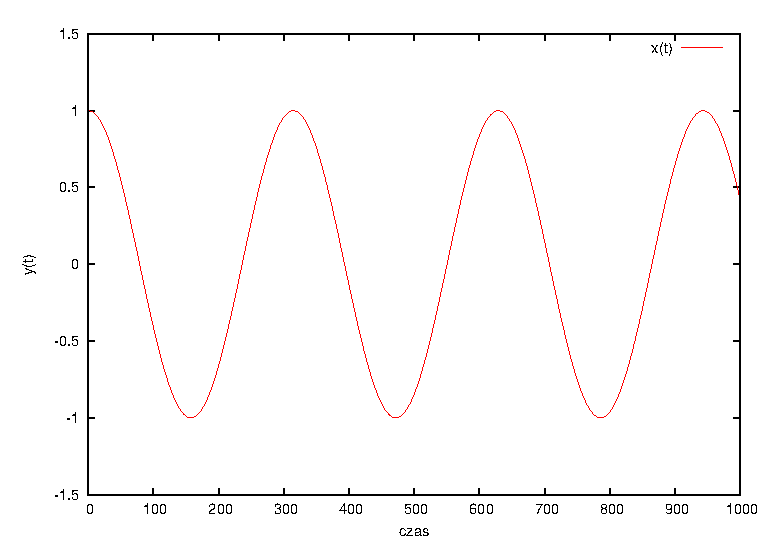
\includegraphics{plot1.eps}
\end{figure}
\item $\beta=0.4, F_0=0.0, \Omega=0.8$\\
wynik czego przedstawia rys. \ref{fig:plot2}
\begin{figure}
\caption{Plot2}
\label{fig:plot2}
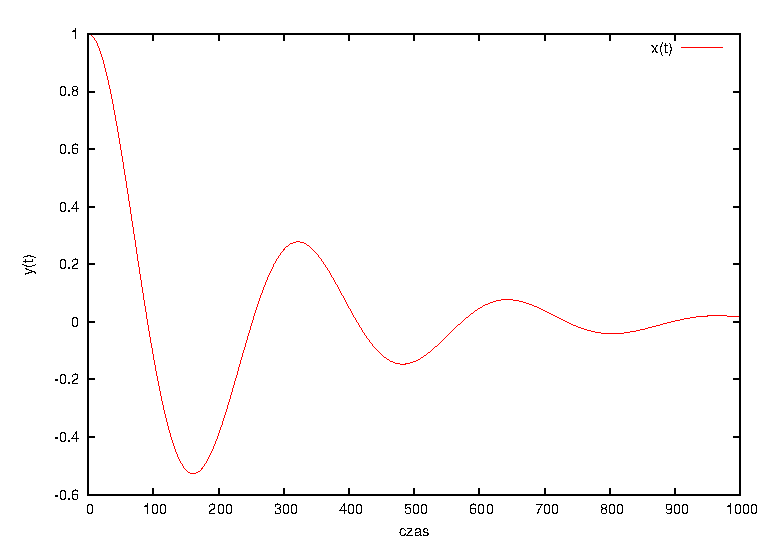
\includegraphics{plot2.eps}
\end{figure}
\item $\beta=0.4, F_0=1.0, \Omega=0.8$\\
czego wynik przedstawia rys. \ref{fig:plot3}
\begin{figure}
\caption{Plot3}
\label{fig:plot3}
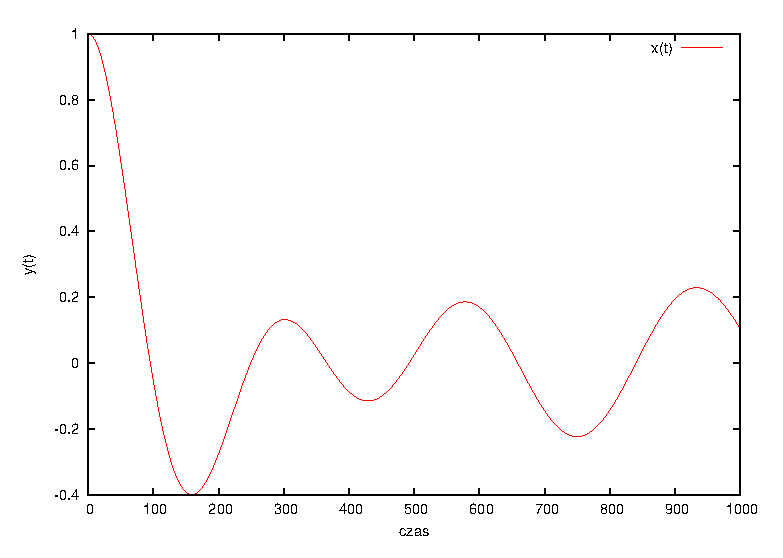
\includegraphics{plot3.eps}
\end{figure}
\end{enumerate}
\item Wnioski\\
Biorąc pod uwagę liczbę operacji wykonywanych podczas działania tego algorytmu, łatwo zauwazyć, że jest on przystosowany do macierzy rzadkich
\end{enumerate}
\end{document}